\section{Clase 8}
\subsection{Generadores de grupos de Lie}
Sea $\M$ una variedad dotada de  sistemas de coordenadas $\{x_i\}_{i=1}^n$,$\{x'_i\}_{i=1}^n$ y sea $G$ un grupo $r$-paramétrico $a_\nu,\, \nu=1,...,r$. La acción del grupo $G$ sobre la variedad $\M$ es dada por el grupo de transformaciones 
\begin{equation}
  x'=f(x,a)  x'_i=f_i(x_j,a_\n )
\end{equation}
\begin{equation}
  x'_i=f_i(x_1,x_2,...,x_n; a_1,a_2,...,a_r)
\end{equation}
Para clarificar ideas consideremos el ejemplo de una variedad $\M$ de $2$ dimensiones que admite las coordenadas $x:(x_1,x_2)$ y $x':(x'_1,x'_2)$ y un grupo uni-paramétrico $G=SO(2)$ de rotaciones en el plano,

\begin{figure}[h!]
	\centering
	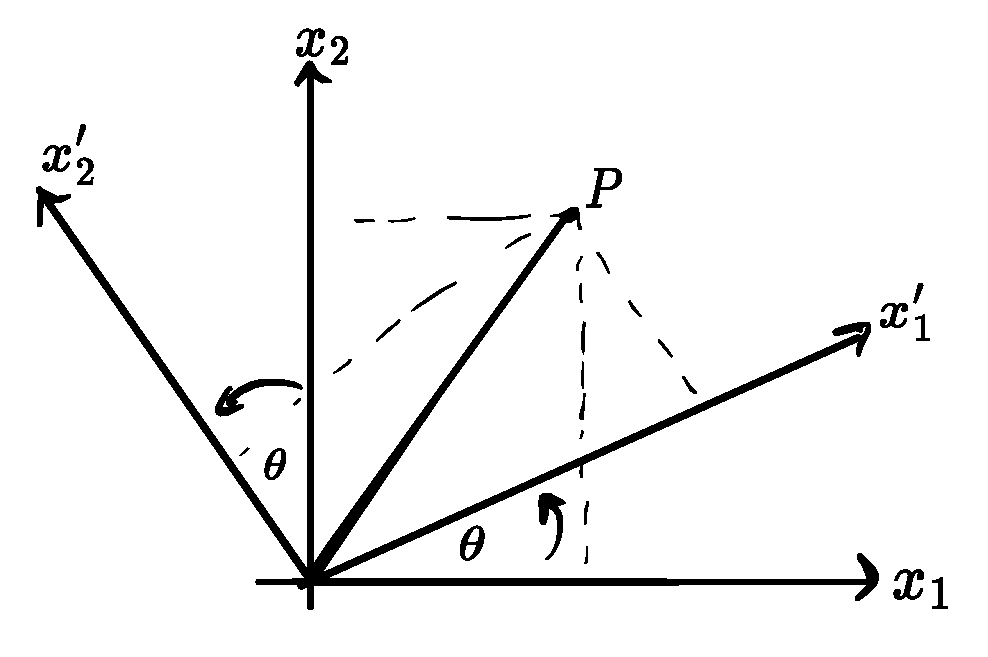
\includegraphics[scale=0.5]{fig/sistema-coord.pdf}
\end{figure}

\begin{align}
  x'_1&=\cos\th x_1-\sin\th x_2\\
  x'_2&=\sin\th x_1+\cos\th x_2
\end{align}
o de manera equivalente
\begin{equation}
  \underbrace{\mqty(x_1'\\x'_2)}_{x'}=\underbrace{\mqty(\cos\th&-\sin\th\\\sin\th&\cos\th)}_{R(\th)}\underbrace{\mqty(x_1\\x_2)}_{x}
\end{equation}

\begin{equation}
  \implies x'=R(\th ) x \longleftrightarrow x'=f(x,\th )x
\end{equation}
o en general
\begin{equation}
  \implies x'=R(a ) x \longleftrightarrow x'=f(x,a )x
\end{equation}
De aquí vemos:
\begin{enumerate}
	\item La acción de $G=SO(2)$ es rotar las coordenadas de $\M$.
	\item Si el ángulo de rotación es pequeño, entonces el cambio experimentado por las coordenadas es también pequeño. Esto implica que en general, un pequeño cambio en los parámetros del grupo induce cambios pequeños en las coordenadas de $\M$.
\end{enumerate}

Notemos que cuando $\th =0$,
\begin{equation}
  R(0)=\mqty(1&0\\0&1)\implies \mqty(x'_1\\x'_2)=\mqty(1&0\\0&1)\mqty(x_1\\x_2)
\end{equation}
es decir,
\begin{equation}
  x'_1=x_1\quad x'_2=x_2
\end{equation}
\begin{equation}
  x'=R(0)x=x,\qquad  x'=f(x,0)=x
\end{equation}




Teniendo en cuenta que en el estudio de los grupos de Lie basta con estudiar su comportamiento infinitesimal, consideremos la expansión infinitesimal de la transformación $x'=f(x,a)$ alrededor de $a=0$.

\begin{equation}
  x'=f(x,a)=f(x,0)+\eval{\pdv{f(x,a)}{a}}_{a=0}\dd a+\cdots
\end{equation}
\begin{equation}
  x'_i=f_i(x_j,a_\n )=f_i(x_j,0)+\pdv{f_i(x_j,0)}{a_\nu }\dd a_\nu
\end{equation}
\begin{equation}
  x'=x+\pdv{f(x,a)}{a}\dd a
\end{equation}
\begin{equation}
  x'_i=x_i+\pdv{f_i(x,0)}{a_\nu}\dd a_\nu
\end{equation}
Esto implica que
\begin{equation}
  \dd x'=\pdv{f(x,0)}{a}\dd a,\qquad \dd x'_i=\pdv{f_i(x,0)}{a_\nu}\dd a_\nu
\end{equation}
Definiendo por comodidad
\begin{equation}
  u(x)=\pdv{f(x,0)}{a},\qquad u_{i\nu}(x)=\pdv{f_i(x,0)}{a_\nu}
\end{equation}
Así,
\begin{equation}\label{8.dxuda}
  \dd x=u(x)\dd a,\qquad \dd x_i=u_{i\nu}\dd a_\nu
\end{equation}
Notar que, de lo anterior\footnote{No estamos siendo estrictos con la posición de los índices coordenados de momento.}
\begin{equation}
 \boxed{ \dv{x_i}{a_\nu}=u_{i\nu}(x)}
\end{equation}
También podemos escribir
\begin{equation}
  \dd x_i=\sum _\n u_{i\nu }(x)\dd a_\n \qquad i=1,2,...,n,\qquad \n =1,2,...,r
\end{equation}

\begin{defi}
	Sea $F(x)=F(x_1,...,x_n)$ una función definida sobre la variedad $\M$. La función $F(x)$ es \textbf{invariante} bajo el grupo de transformaciones \begin{equation}
  x'=f(x,a)
\end{equation}
si $$F(x')=F[f(x,a)]=F(x).$$
\end{defi}

Consideremos ahora el cambio experimentado por la función $F(x)$ cuando cambian las coordenadas $x$ debido a un cambio en los parámetros del grupo.

Bajo un cambio en $x$ se tiene que $F(x)$ cambia como\footnote{El cambio en el parámetro genera un cambio en las coordenadas, y el cambio en las coordenadas genera un cambio en la función $F(x)$.}
\begin{align}
  \dd F&=\pdv{F}{x}\dd x=\pdv{F}{x}u(x)\dd a\\
  \dd F&=\dd a \l(u(x)\pdv{x}\r)F\\
  \dd F&=\dd a_\n \left(u_{i\n }(x)\pdv{x_i}\right)F
\end{align}
donde hemos usado \eqref{8.dxuda}.
\begin{defi}
	Se define el \textbf{generador} del grupo como el operador dado por
	\begin{equation}
  \boxed{X_\n =\sum_i u_{i\n }\pdv{x_i}},\qquad i=1,2,...,n,\qquad \n =1,2,...,r
\end{equation}
\end{defi}
Así, existe un generador por cada parámetro del grupo.

Esto implica que
\begin{equation}
  \dd F=\dd a_\n X_\n F\equiv XF
\end{equation}
donde
\begin{equation}
  X=\dd a_\n X_\n \equiv \dd a^\n X_\n 
\end{equation}

\begin{obs}
	Los generadores $X_\n$ son operadores que pueden o no ser operadores hermíticos. En el caso que ellos no sean hermíticos, pueden ser convertidos en hermíticos en general, multiplicándolos por $i$.
\end{obs}

\begin{teor}
	A partir de un conjunto de operadores hermíticos $X_\n$ podemos obtener una representación del grupo por medio de operadores unitarios
	\begin{equation}
 \boxed{U(a_\n )=e^{i a_\n X_\n }}
\end{equation}
\end{teor}

\begin{teor}
	Si $X_\n$ y $X_\m$ son generadores de un grupo de Lie, entonces
	su conmutador es una combinación lineal se dichos generadores:
	\begin{equation}
  [X_\n,X_\m ]=C_{\n\m}^{~~\lambda} X_\lambda \equiv C_{\m\n\lambda }X_\lambda
\end{equation}
donde
\begin{equation}
  C_{\n\m}^{~~\lambda}=-C_{\m\n }^{~~\lambda}
\end{equation}
\end{teor}
Dado que este producto es antisimétrico, satisface la \textbf{identidad de Jacobi},
\begin{equation}
  [[X_\m,X_\n ],X_\lambda]+[[X_\lambda,X_\m  ],X_\n ]+[[X_\n,X_\lambda ],X_\m ]=0
\end{equation}

\begin{ej}
	Consideremos el siguiente grupo de transformaciones 
	\begin{equation}\label{8.1}
  x'=\a_1x+\a_2,\qquad \a=(\a_1,\a_2)
\end{equation}
\begin{itemize}
	\item Encuentre los generadores del grupo
	\item Determine sus relaciones de conmutación
\end{itemize}
\end{ej}

\begin{sol}
	De \eqref{8.1} vemos que la identidad del grupo es dada por $\a_1=1$ y $\a_2=0$ ya que $x'=1x+0=x$, lo que implica que $\a_0=(\a_1^0,\a_2^0)=(1,0)$. Con el objeto de tener una identidad nula, definimos
	\begin{equation}
  a_1=\a_1-1,\qquad a_2=\a_2
\end{equation}
Es decir,
\begin{equation}
  a_1^0=\a_1^0-1,\qquad a_2^0=\a_2^0
\end{equation}
\begin{equation}
	\implies a_1^0=1-1=0,\qquad a_2^0=0
\end{equation}
\begin{equation}
  \implies a_0=(a_1^0,a_2^0)=(0,0)
\end{equation}
Así, el grupo de transformaciones toma la forma
\begin{equation}
  x'=(1+a_1)x+a_2
\end{equation}
\begin{equation}
  \implies\boxed{ x'=f(x,a)=x+a_1 x+a_2}
\end{equation}
\begin{equation}
  \implies \dd x_i=\pdv{f_i(x,0)}{a_\n }\dd a_\n =\uin \dd a_\n 
\end{equation}
\begin{equation}
  \dd x_i=\sum_\n \pdv{f_i}{a_\n }\dd a_\n 
\end{equation}
\begin{equation}
  \dd x_1\equiv \dd x=\pdv{f}{a_1}\dd a_1+\pdv{f}{a_2}\dd a_2
\end{equation}
\begin{equation}
  \dd x=x\dd a_1+1\dd a_2
\end{equation}
\begin{equation}
  \boxed{\dd x=x\dd a_1+\dd a_2}
\end{equation}
pero
\begin{equation}
  \dd x=u_{11}\dd a_1+u_{12}\dd a_2
\end{equation}
\begin{equation}
  \implies u_{11}=x,\qquad u_{12}=1
\end{equation}
de manera que 
\begin{equation}
  X_{\n }=\sum_i \uin \pdv{x_i}
\end{equation}
\begin{equation}
  X_1=u_{11}\pdv{x_1}=u_{11}\pdv{x}=x\pdv{x}
\end{equation}
\begin{equation}
  X_2=u_{12}\pdv{x_1}=u_{12}\pdv{x}=\pdv{x}
\end{equation}
Así, los generadores del grupo son
\begin{equation}
  X_1=x\pdv{x},\qquad X_2=\pdv{x}
\end{equation}
El conmutador es
\begin{align}
  [X_1,X_2]f&=X_1X_2f-X_2X_1f\\
  &=x\pdv{x}\left(\pdv{f}{x}\right)-\pdv{x}\left(x\pdv{f}{x}\right)\\
  &=x\pdv[2]{f}{x}-\pdv{f}{x}-x\pdv[2]{f}{x}\\
  &=-\pdv{f}{x}\\
  &=-X_2 f
\end{align}
\begin{equation}
  \implies [X_1,X_2]=-X_2
\end{equation}
Dado que
\begin{equation}
  [X_1,X_2]=C_{12}^{~~1}X_1+C_{12}^{~~2}X_2
\end{equation}
se tiene que las constantes de estructura son
\begin{equation}
  C_{12}^{~~1}=0,\qquad C_{12}^{~~2}=-1
\end{equation}
\end{sol}

\subsection{Grupos matriciales}
Sea $\M$ una variedad que admite las bases\footnote{Ver Ref. \cite{book:176834}} $\{\hat{e}_i\}_{i=1}^n$,$\{\hat{e}'_i\}_{i=1}^n$ y $\{\hat{e}''_i\}_{i=1}^n$ asociadas a las coordenadas $\{x_i\}_{i=1}^n$,$\{x'_i\}_{i=1}^n$ y $\{x''_i\}_{i=1}^n$. Un cambio de base es dado por
\begin{equation}
  \he'_j=B_j^{~i}\he_i,\qquad \he''_k=A_k^{~j}\he '_j,\qquad \he''_k=C_k^{~i}\he _i
\end{equation}
es decir,
\begin{equation}
  \he''_k=A_k^{~j}B_j^{~i}\he'_i=C_k^{~i}\he _i
\end{equation}
\begin{equation}
  \implies \boxed{C_k^{~i}=A_k^{~j}B_j^{~i}}
\end{equation}
Todas las bases de un espacio vectorial están relacionadas por medio de matrices. El conjunto de estas matrices constituyen un grupo.

\begin{defi}
	El conjunto de matrices $n\times n$ invertible que definen un cambio de base constituyen un grupo conocido como \textbf{grupo lineal general} definido sobre los espacios $\mathbb{R}^n,\mathbb{C}^n,\mathbb{Q}^n$. Estos grupos son denotados por $GL(n,\mathbb{R}),\, GL(n,\mathbb{C}),\, GL(n,\mathbb{Q})$.
\end{defi}

\subsubsection{Grupo general lineal $GL(n,\mathbb{C})$}
Grupo compuesto por todas las matrices complejas invertibles $n\times n$.

 Toda matriz $A\in GL(n,\mathbb{C}^n)$ tiene $2n^2$ elementos ($n^2$ elementos reales y $n^2$ elementos imaginarios).
 
 Este grupo tiene $2n^2$ parámetros reales, por lo cual tiene dimensión $2n^2$.
 
 \subsubsection{Grupo general lineal real $GL(n,\mathbb{R})$}
 Si exigimos que las matrices de $GL(n,\mathbb{C}^n)$ sean todas con elemento reales, obtenemos el grupo lineal general real $GL(n,\mathbb{R}^n)$, el cual tiene $n^2$ parámetros reales.
 
 \subsubsection{Grupo general lineal especial $SL(n,\mathbb{C})$}
 Si exigimos que todas las matrices de $GL(n,\mathbb{C})$ satisfagan las condiciones que tengan determinante $+1$, entonces obtenemos el grupo lineal especial $SL(n,\mathbb{C})$. Así, si $A\in SL(n,\mathbb{C})$, entonces $\det A=1$.
 
  \subsubsection{Grupo general lineal especial real $SL(n,\mathbb{R})$}
Si exigimos que todas las matrices de $GL(n,\mathbb{R})$ tengan determinante $+1$ entonces obtenemos el grupo especial lineal real $SL(n,\mathbb{R})$.









































